\section{Introducción}

De cara a desarrollar el proyecto final para la asignatura hemos decidido escoger el problema de reentrenar una red neuronal convolucional ya preentenada con un conjunto de datos (en nuestro caso ImageNet) para resolver otro problema distinto.

En concreto hemos escogido esta temática ya que nos parecía muy interesante el problema de transferencia de conocimiento de una RNN. Actualmente estamos viendo como se están desarrollando múltiples redes neuronales convolucionales que son capaces de resolver gran cantidad de problemas, sin embargo, como vimos en la práctica dos de la asignatura, es muy común el reutilizar una red para otro problema distinto al entrenado, ya sea utilizando sus parámetros si se tratan de problemas similares, reentrenando la red completa, o haciendo un fine tuning debido al coste computacional que conlleva entrenar una red neuronal convolucional desde cero. Por este motivo nos hemos interesado en estudiar más a fondo este problema, así como intentar aplicarlo a un problema que habitualmente no es muy tratado, la detección de un tipo de platos de comida concretos.


\vspace{5 mm}

\subsection{Motivación}

\vspace{5 mm}

El principal motivo por el que queremos desarrollar una CNN que reconozca platos de comida, concretamente platos de la cocina tradicional Vietnamita, es que no se trata de un campo muy explotado dentro de la clasificación de imágenes.

\vspace{3 mm}

Hay muchos papers que hablan de CNN para la clasificación de comida, donde se suele utilizar el famoso dataset \textbf{Food-101} para su entrenamiento. Estas CNN reconocen los platos de cómida más \textit{típicos} a nivel mundial, pero lo interesante y por lo que estamos haciendo este trabajo, es ver cómo podemos hacer que una CNN que reconozca estos platos \textit{típicos}, reconozca también platos tan concretos como los de la cocina Vietnamita.

\vspace{3 mm}

La Singapore Management University (SMU) desarrolló en el año 2017 una CNN llamada \textbf{foodai} capaz de reconocer 756 clases de comida entre las que había platos e ingredientes individuales. Si le pasamos a esta CNN la siguiente imagen la clasificaría sin problema como \textbf{Fried Pork Chop}:

\vspace{5 mm}

\begin{figure}[H]
  \centering
  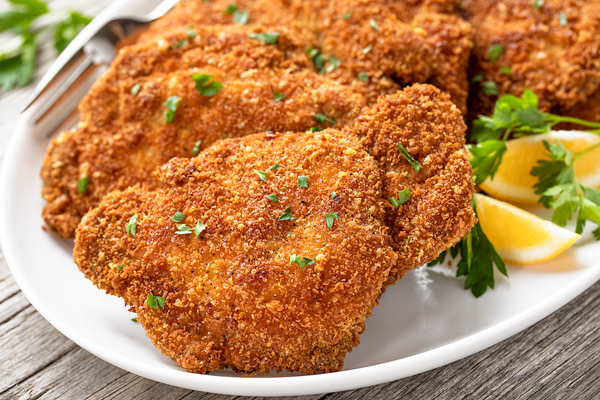
\includegraphics[width=0.5\linewidth]{Imagenes/empanada.jpeg}
  \caption{Fried Pork Chop}
  \label{fig:sub-first}
\end{figure}

Pero, ¿qué pasaría si le pasamos a la CNN un plato típico de la comida Vietnamita como puede ser el \textbf{Bun Bo Hue}?

\vspace{5 mm}

\begin{figure}[H]
  \centering
  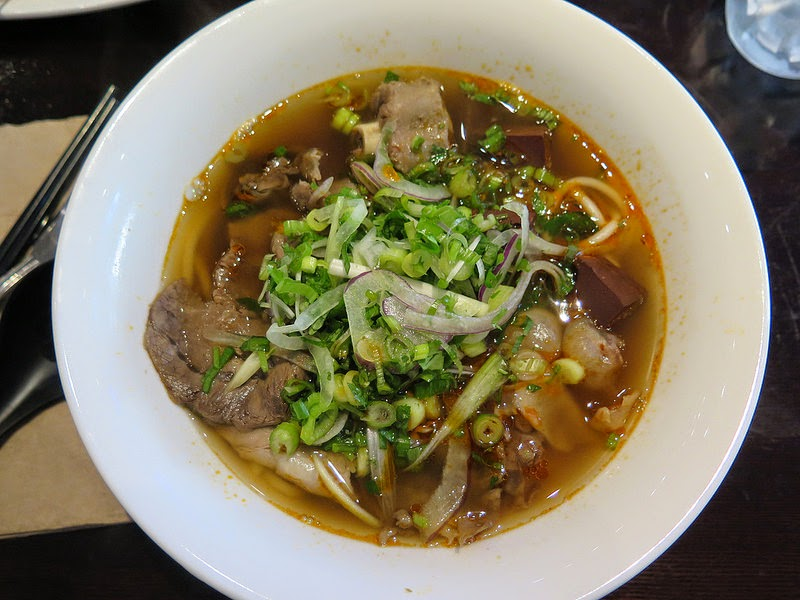
\includegraphics[width=0.5\linewidth]{Imagenes/bunbohue.jpeg}
  \caption{Bun Bo Hue}
  \label{fig:sub-first}
\end{figure}

\vspace{5 mm}

La CNN no habrá sido entrenada con la clase \textbf{Bun Bo Hue} y por lo tanto no podrá clasificar el plato correctamente, por lo que lo clasificará en una clase parecida.

\vspace{3 mm}

Es por todo lo anterior que queremos desarrollar una CNN que reconozca platos típicos de la comida Vietnamita, al igual que platos más \textit{generales} y otras clases pertenecientes al dataset \textbf{ImageNet}.

\newpage

\subsection{Pasos a seguir para conseguir nuestro objetivo}

De cara al desarrollo del proyecto comenzaremos con una introducción teórica a las redes neuronales convolucionales, tanto de su funcionamiento teórico como de la herramienta que utilizaremos para el desarrollo del proyecto, Keras. Tras la explicación de los fundamentos teóricos hablaremos del estado del arte de este problema, el cuál se ha estado desarrollando los últimos años; que se ha llegado a conseguir similar a nuestro problema, y que diferencias principales hay entre esos avances y nuestro problema concreto.

Como se nos ha recomendado, de cara a desarrollar nuestro proyecto, la base del estado del arte será fundamental ya que nos permitirá conocer que puede funcionar o no para nuestro problema concreto, además de dar un apoyo teórico y práctico más fuerte a la hora de realizar el trabajo sin tratarse simplemente de un ajuste fino como hicimos en la práctica dos de la asignatura.

Esto lo podremos llevar a cabo debido a que, aunque el problema de clasificar comida no es muy habitual, podemos encontrar algunos casos concretos en los que se ha avanzado bastante como FoodAI, o algunas redes neuronales preparadas para reconocer la base de imágenes Food101 que aunque se traten de problemas más genéricos que el nuestro nos pueden ayudar para el problema de la detección de un tipo concreto de comida.
